%%%%%%%%%%%%%%%%%%%%%%%%%%%%%%
%
%
%\BiChapter{相关理论}{Related Theories}
%\BiSection{光场技术基本理论}{Basic Theory of Light Field Technology}

%\BiSubsection{光场成像原理}{Principles of Light Field Imaging}

%\BiSubsection{光场数据的可视化}{Visualization of Light Field Data}
%
%\BiSection{光场显著性目标检测相关理论}
%{Related Theories on Light Field Salient Object Detection}
%
%\BiSubsection{基于多视角图像的显著性目标检测原理}
%{Principles of Salient Object Detection via Multi-view Images}
%
%\BiSubsection{基于焦点堆栈的显著性目标检测原理}
%{Principles of Salient Object Detection via Focus Stack}
%
%\BiSubsection{显著性目标检测性能评估指标}
%{Performance Evaluation Metrics for Salient Object Detection}
%
%
%%%%%%%%%%%%%%%%%%%%%%%%%%%%%%


\BiChapter{相关理论}{Related Theories}
\label{chap:part2}

\BiSection{光场技术基本理论}{Basic Theory of Light Field Technology}

光场的概念最早由A.Gershun~\cite{gershun1939light}教授提出,是空间中光线集合的完备表示,采集并显示光场就能在视觉上重现真实世界。
1991年,MIT的Edward H.Adelson教授和James R.Bergen\cite{adelson1991plenoptic}教授指出人眼对光线的视觉感知可以认为是沿着单一函数的一个或多个方向的局部变化,描述了光照射到观察面的信息结构。
一旦定义了这个函数,各种潜在的视觉属性(如运动、颜色和方向)的测量就能够自动分离出来。
这个函数被称为全光函数,表示为:
%$$$$
\begin{equation}
	P(x,y,z,\theta,\varphi,\lambda,t)
\end{equation}\par
其中$(x,y,z)$为发光物体的空间位置,$(\theta,\varphi)$分别表示传播光线入射的垂直角度和水平角度,$\lambda$表示传播光线的波长,发光物体所发射的光线信息随时时间$t$的推移而变化。
然而,这种能够记录空间中光线信息的七维全光函数过于复杂、数据量大,难以记录和存储,在实际计算中并未得到应用。
需要对其进行简化处理。
McMillan等~\cite{mcmillan2023plenoptic}在七维全光函数的基础上提出了
简化波长$\lambda$和时间$t$的更为方便的五维光场模型。
\begin{equation}
	P(x,y,z,\theta,\varphi)
\end{equation}\par
五维光场模型通过记录红、绿、蓝三原色来简化波长$\lambda$,以及通过记录不同帧来简化时间$t$。
实际上,光线在空间传播中,因传播距离而造成的信息损耗微乎其微,光场模型还可以进一步简化。
%如果不考虑光线在空间传播过程中的衰减,记录光场信息的五维模型还可以进一步简化成四参数光场函数。
%\par
%
%
%
%
\begin{figure}[!ht]
	\centering
	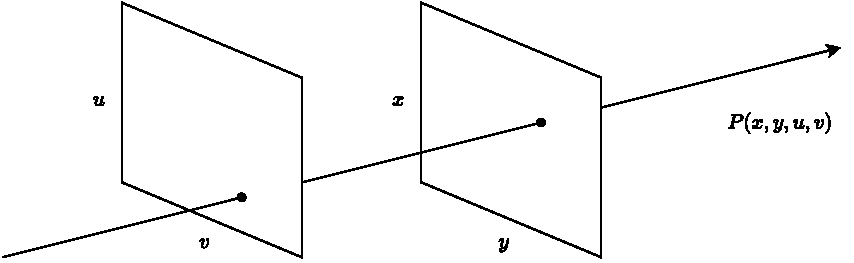
\includegraphics[width=0.95\linewidth]{figures/chapter2/double_plane_model.drawio}
	\bicaption{光场双平面四参数模型}{Light field biplane four-parameter model}  
	\label{chapter2_fig1:double_plane}
\end{figure}
%
%
%
%
Levoy等~\cite{levoy2023light}忽略掉传播距离维度$z$得到四维光场模型,
同时提出光场渲染理论和双平面模型来描述静态的可见光。
双平面模型利用两个互相平行的参数化平面表示四维光场。
假设光线在没有遮挡物和散射介质的区域,忽略光线在传播过程中波长和时间维度的变化,
则任意一个包含位置和方向信息的光线都可以用双平面参数来表示,
空间中的光线穿过这两个平面分别相交于点$(u, v)$和点$(s, t)$,
光线即可用四维光场函数表示,如图~\ref{chapter2_fig1:double_plane}~所示,其模型参数如下:
\begin{equation}
	P(u, v, x, y)
\end{equation}\par
在光场成像设备中,我们可以用$(u, v)$表示光线与微透镜阵列的交点,用$(s, t)$表示光线与CCD传感器探测面的交点。一条光线在整个四维空间中对应着光场的一个采样点。四维光场理论的推出为全光相机、相机阵列等设备提供了理论基础。目前,大多数单体全光相机和相机阵列的光场采集设备都遵循着四维光场理论。
%
%
%发展出了适用于光学系统的光场双平面参数特征。
%假设一条光线在两个不共面的平面$(u,v)$和平面$(s,t)$各有一个交点,则该光线可以用这两个交点唯一表示。
% \emph{et~al.}~
%光场是计算机科学领域的学者定义的“Light Field”,是指除了包含原图像矩阵中的空间坐标$(x,y)$和强度$I$外,还有光线入射的角度信息$(\theta,\varphi)$。
%光在传播过程中的各种潜在的视觉属性(如运动、颜色和方向)。




%%%%%%%%%%%%%%%%%%%%%%%%%%%%%%%%%%%%%%%%%%%%%%%%%%%%%%%%%%%%%%%%%%%%%%%%%%%%
\BiSubsection{光场成像原理}
{Principles of Light Field Imaging}

在传统成像中,光线被捕获并呈现到成像平面上。然而,光场成像采用不同的方式。
它是一种计算成像技术,旨在捕获光线强度的同时记录光线的传播方向。
为了得到可视化的图像信息,必须对捕获的光场信息进行计算处理。
根据成像设备或记录方法的不同,现有的光场成像方式可以分为多传感器采集成像、
时间序列采集成像、空域复用成像和频域复用成像。\par
%
%
%
%
\begin{figure}[!ht]
	\centering
	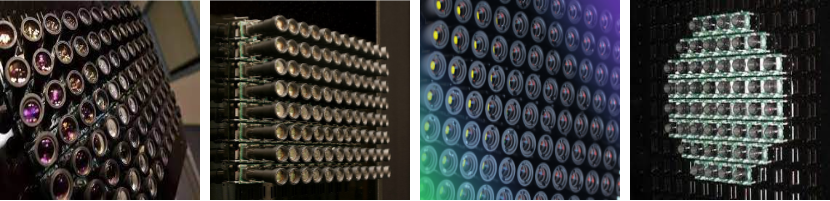
\includegraphics[width=1\linewidth]{figures/chapter2/camera_array}
	\bicaption{相机阵列光场成像}{Camera array for light field imaging}  
	\label{chapter2_fig2:camera_array}
\end{figure}
%
%
%
%
(1)使用相机阵列获取光场信息是通过多个相机以特定的空间分布在不同视角下捕获场景图像的方法,
如图~\ref{chapter2_fig2:camera_array}~所示。
每个相机捕获的是四维光场在其相对于场景方向上的二维投影。
通过融合这些相机捕获的图像,就可以获得完整的四维光场数据。
大尺度空间相机阵列主要应用于合成孔径成像以实现“透视”监测,或通过拼接实现大视角全景成像。
相比之下,紧密排列的相机阵列则主要用于捕获高性能动态场景或场景的三维分布和结构等信息。
光场数据的空间解析度取决于传感器本身,而角度解析度由传感器数量和布局方式确定。
这种采集方法能够在单次曝光中瞬时捕捉光场,因此还能记录光场的时间序列信息。
尽管这种成像方法空间解析度较高,但却带来了庞大的图像数据量,因此处理上更加耗时。
此外,这种成像方式对多传感器的相对位置要求也较高。\par
%
%
%
%
\begin{figure}[!ht]
	\centering
	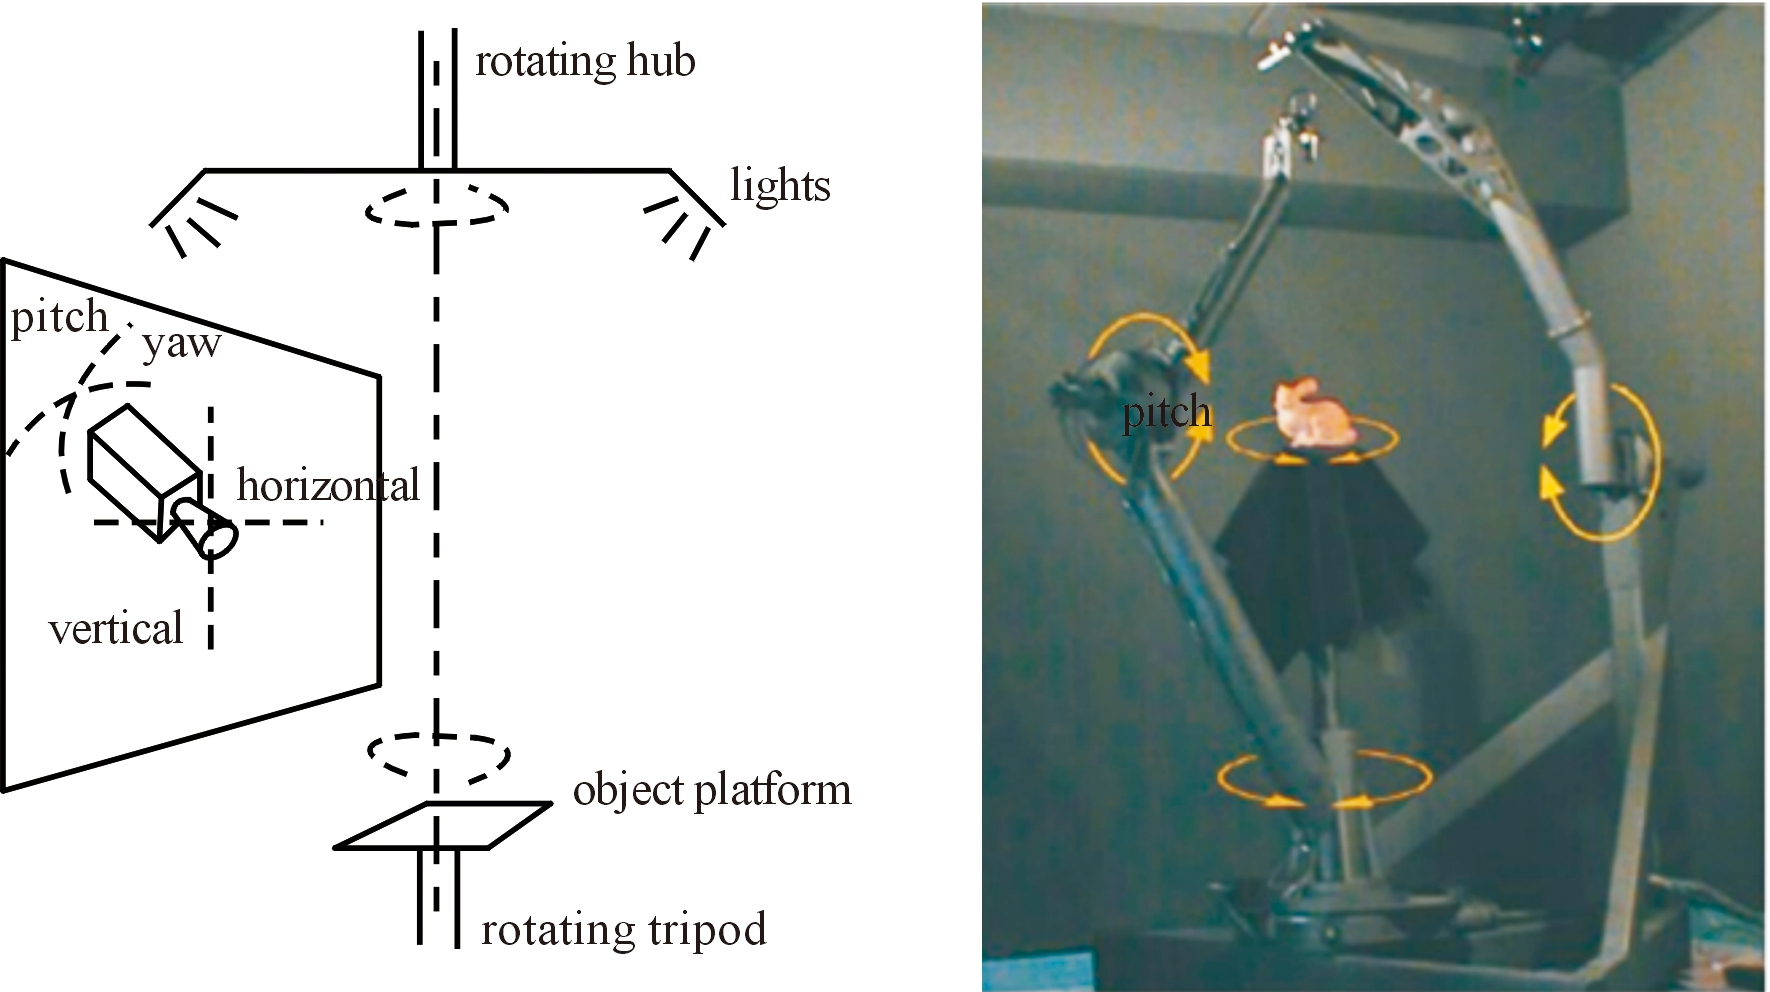
\includegraphics[width=0.7\linewidth]{figures/chapter2/time_seq2}
	\bicaption{时间序列光场成像}{Time-series light field imaging}  
	\label{chapter2_fig3:time_seq2}
\end{figure}
(2)除了多个相机阵列排布外,Marc Levoy等人\cite{levoy2023light}采用了单相机扫描系统。
他们通过让相机在固定的导轨上移动,分时获取不同空间视角下的场景图像,
最后将这些图像进行融合,从而实现相同的功能。
图~\ref{chapter2_fig3:time_seq2}~是典型的时序采集光场信息的示例。
与多传感器采集相比,这种方法的优势在于能够实现高密度角度分辨率的光场信息采集。
然而,缺点也显而易见,即需要高精度的控制,并且相对于多传感器采集,这种成像方式也更加耗时。
这些缺点限制了该成像方式仅适用于静态场景的光场信息采集。\par
%
%
%然而,由于需要进行扫描,这种方法更适用于静态场景的光场测量。
%此外,测量的精度受到相机移动定位精度的影响。
% 图3和图4展示了相机阵列以及单相机路径扫描方案实现光场信息获取的示例。
%
%
%
\begin{figure}[!ht]
	\centering
	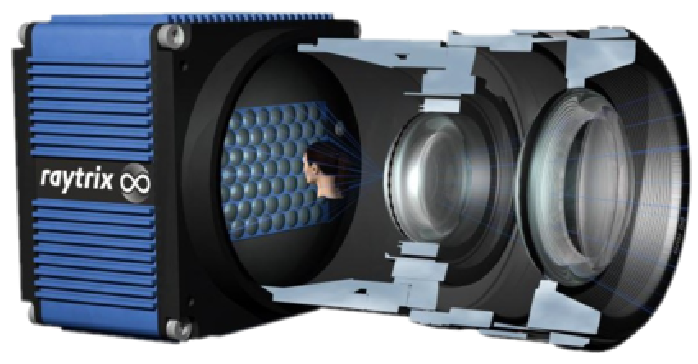
\includegraphics[width=0.65\linewidth]{figures/chapter2/microlens_for_lf_imaging2.drawio}
	\bicaption{微透镜光场成像}{Microlens light field imaging}  
	\label{chapter2_fig4:microlens_for_lf_imaging}
\end{figure}
(3)空域复用的成像方式通过在图像传感器上安装微透镜阵列来实现,这是光场采集中常见的方式之一。
图~\ref{chapter2_fig4:microlens_for_lf_imaging}~展示了这种空域复用的成像方式的工作原理:通过将微透镜阵列插入普通成像系统的主透镜的一次像面,每个微透镜单元及其对应的传感器区域记录了光线从不同视角成像的集合,从而获得包含位置和传播方向的四维光场数据。
空域复用的成像方式优势在于结构紧凑,一次曝光即可捕捉光线强度与方向,适用于不同场景和动态场景的光场信息采集。
1992年,Adelson~\cite{adelson1992single}及其团队首次提出了利用微透镜阵列的光场相机模型;
然而,这种空域复用方式需要在空间分辨率和角度分辨率之间进行权衡。
当角度分辨率最大时,微透镜与图像传感器重合,空间分辨率最小;反之亦然。
为解决这一问题,
Georgiev~\cite{georgiev2010focused}在2021年提出了可调整微透镜与图像传感器相对位置的聚焦光场相机结构,
实现了角度分辨率与空间分辨率的动态调整。
%
% 相机阵列的体积庞大,限制了其应用范围。
% 通过缩小相机阵列中各成像单元之间的基线,可以在单个相机框架下利用微透镜阵列来采集光场信息。
% 空域复用的成像方式通过在图像传感器上安装微透镜阵列来实现,这是光场采集中常见的方式之一,可通过单次曝光捕获光场信息。
%
%



%%%%%%%%%%%%%%%%%%%%%%%%%%%%%%%%%%%%%%%%%%%%%%%%%%%%%%%%%%%%%%%%%%%%%%%%%%%%
\BiSubsection{光场数据的可视化}{Visualization of Light Field Data}

根据先前的描述,四维模型中双平面光场模型是目前广泛采用的光场模型,其中两个维度表示空间位置,另外两个维度表示方向角度。
在三维世界中,描绘四维光场数据是具有挑战性的,可以通过固定双平面光场模型的任意两个维度来展示二维切片以可视化光场数据。
虽然二维光场切片无法传达完整的光场信息,但可以帮助解释光场数据的内在特征。
固定角度维度可以获得子孔径图像阵列形式的光场数据;固定空间维度可以获得宏像素形式的光场数据;固定一个角度维度和一个空间维度可以获得包含空间和角度信息的 EPI 形式的光场数据。焦点堆栈数据也是一种光场可视化的形式。
常用的光场可视化方式主要有子孔径图像阵列形式、宏像素形式、极线图形式和焦点堆栈。
\par
%
% %常用的光场可视化方式主要有多视角图像、极平面图像和焦点堆栈3种。
%
%
(1)
子孔径图像阵列视图是广泛使用的光场可视化方法之一。
固定角度维度$(u, v)$,令$u = u^{*}$,$ v = v^{*} $,
则$P(u^{*}, v^{*}, x, y) $表示在单个视点$(u^{*}, v^{*})$下的图像$(x,y)$。
若把$(x,y)$看成传统相机所成的像,$(u, v)$就表示相机所在的位置。
光场$P(u, v, x, y)$就可以理解为相机在视点平面等间隔采样,表现为相机不同视点$(u, v)$位置处所捕获的图像。
光场相机在不同视点下捕获的图像称为子孔径图像,又被称为亚光圈图像,简称为视图。
因此,四维光场数据可以被呈现为子孔径图像的阵列形式,如图~\ref{chapter2_fig5:multi_photo}~所展示。
图中右侧显示了以中心视点(5, 5)为基准的子孔径图像的放大示意图。\par
%
%
\begin{figure}[!ht]
	\centering
	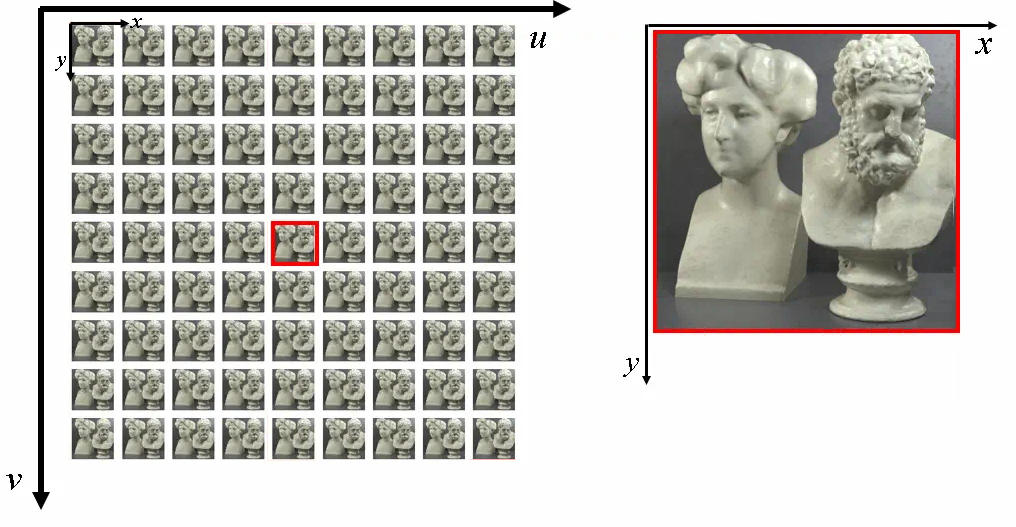
\includegraphics[width=0.75\linewidth]{figures/chapter2/multi_photo}
	\bicaption{子孔径图像阵列形式的光场数据可视化}
	{Visualization of light field data in the form of subaperture image arrays}  
	\label{chapter2_fig5:multi_photo}
\end{figure}
%
%
%
%
\begin{figure}[!ht]
	\centering
	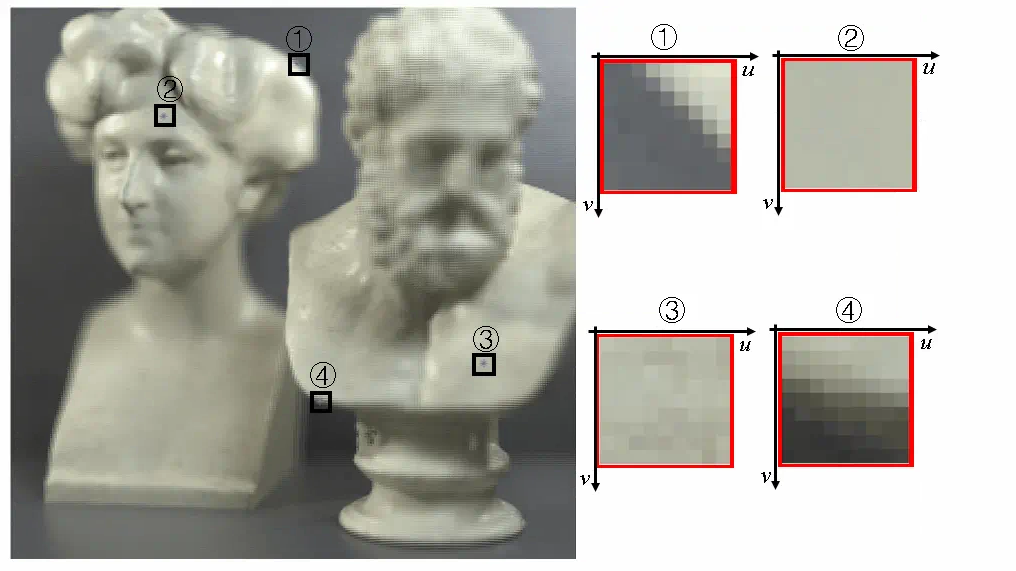
\includegraphics[width=0.80\linewidth]{figures/chapter2/macro_photo}
	\bicaption{宏像素形式的光场数据可视化}
	{Visualizing light field data in macropixel form}  
	\label{cpt2_fig5:macro_photo}
\end{figure}
%
%
%multi_photo
%
%
(2)
宏像素视图是另一种光场可视化形式。固定空间维度的坐标$(x, y)$,令$x=x^{*}$,$y=y^{*}$,
则$ P(u, v, x^{*}, y^{*})$可以表示为单个宏像素,
通过按照空间分辨率遍历所有宏像素,并按照图像顺序排列,形成宏图像。
如图~\ref{cpt2_fig5:macro_photo}~所示。
每个宏像素在宏图像中的分辨率代表了光场的角度分辨率。
%
不考虑遮挡的情况,$ P(u, v, x^{*}, y^{*})$表示场景中某一物点在所有视点下对应的像素值,
即$ P(u, v, x^{*}, y^{*})$表示光场采集设备所捕获到的物点发出的所有光线,
如图~\ref{cpt2_fig5:macro_photo}~中标号\ding{193}、\ding{194}的宏像素所示。
考虑遮挡的情况,$ P(u, v, x^{*}, y^{*})$可由场景中的某一遮挡物点,
在可视点下对应的像点和在非可视点下其他物点对应的像点的组合,
在图~\ref{cpt2_fig5:macro_photo}~中标号\ding{192}、\ding{195}的宏像素中,
可以看到宏像素内含有不同物点发出的光线。\par
%
%
%
%
%
\begin{figure}[!ht]
	\centering
	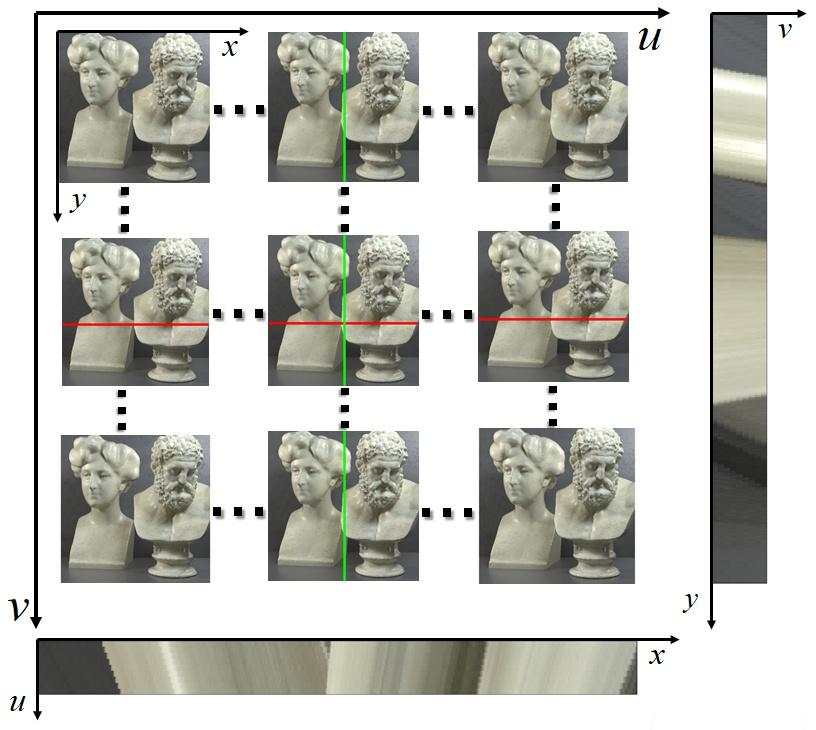
\includegraphics[width=0.75\linewidth]{figures/chapter2/epi_photos}
	\bicaption{极视角形式的光场数据可视化}
	{Light field data visualization in polar perspective form}  
	\label{cpt2_fig6:epi_photos}
\end{figure}
%
%
%
(3)
极平面视图(Epipolar-Plane Images, EPI)是通过固定一个角度维度的坐标和一个空间维度的坐标得到的。
在多视角图像中,固定方向维度的角度域表示法主要用于展示光场的空间信息,
而固定空间维度的多视图表示法则着重于显示光场的方向信息。
相比之下,极平面图像通过固定一个角度坐标和一个空间坐标来展示场景的景深和结构信息。
具体来说,
当固定$(v, y)$坐标,令$v=v^{*}$,$y=y^{*}$,
则$ P(u, v^{*}, x, y^{*})$被称为固定$(v^{*}, y^{*})$的极平面图像,即垂直方向上的EPI图像。
同理,当固定$(u, x)$,则$ P(u^{*}, v, x^{*}, y)$被称为固定$(u^{*}, x^{*})$的极平面图像,
即水平方向上的EPI图像。
如图~\ref{cpt2_fig6:epi_photos}~所示,光场中同一水平视点上所有红色线条所在的行像素堆叠后就形成立下侧的EPI;
类似的,将光场中同一垂直视点上所有绿色线条所在的列像素堆叠后就形成立右侧的EPI。
当物体满足朗伯体表现的性质,即向各个方向发出的光线强度相等时,那么该点在极平面图像中被表示为一条直线,该直线的斜率可以反映出该点的深度信息。\par
%
%
%
%
\begin{figure}[!ht]
	\centering
	
\includegraphics[width=0.95\linewidth]{figures/chapter2/focal_stack}
	\bicaption{焦点堆栈形式的光场数据可视化}
	{Visualization of light field data as focus stack}  
	\label{cpt2_fig7:focal_stack}
\end{figure}
%
%
%
%
(4)
% 焦点堆栈数据是另一中常用的光场数据表示方法。
焦点堆栈数据是利用光场重新聚焦技术综合生成的,也是当前广泛应用的一种数据形式。
光场重新聚焦的核心是利用不同深度的物体在多视角下产生不同视差的原理,
通过平移叠加多视角图像来获得重新聚焦在特定深度的图像。
%
%
%
%
%
具体来说,
对于给定光场的多视角图像,选取某一行或某一列图像,确定特定深度,根据深度和视差的关系计算视差,
在叠加图像时按照该行或该列的顺序进行视差平移并叠加。
在这个过程中,与特定深度对应的物体在平移后与中心视角图像匹配像素,叠加后呈现清晰的聚焦像素,
而不在该深度范围内的物体在平移后匹配到不同像素,
叠加后呈现模糊的散焦像素。
通过选择一组深度,可以生成一组在不同深度聚焦的焦点堆栈数据。
%
%
%
在这些图像中,聚焦于物体深度的部分呈现清晰度,而非聚焦部分则显得模糊。
由于“近大远小”效应,不同图像之间存在放大比例差异。
放大比例记录了光线传播方向的信息,这些存在的放大比例可以进行光场的重投影。
这种特性使焦点堆栈数据包含丰富的场景结构信息,为显著性物体检测工作提供了重要支持。
\par
%
%
%
%\textcolor{red}{TODO}
%
%搜集聚焦堆栈数据的方法包括移动镜头或探测器,以采集在不同成像平面上聚焦的图像序列。在这些图像中,聚焦于物体深度的部分呈现清晰度,而非聚焦部分则显得模糊。由于“近大远小”效应,不同图像之间存在放大比例差异。放大比例记录了光线传播方向的信息,只有在存在放大比例时才能进行光场的重投影;而利用光场重聚焦技术(例如,位移和叠加)生成的重聚焦数据则不包含放大比例信息,能够用于深度重建,但无法重新投影出完整的光场。然而,对于深度重建来说,放大比例本身并无实际帮助。
%
%
%
%当固定x=x0, u=u0时,按照空间和方向的顺序排列在一起,就可以得到垂直方向的EPI图像;当固定y=y0, v=v0时,通过改变x的u的顺序,就能得到水平方向的EPI图像。当物体满足朗伯体表现的性质,即向各个方向发出的光线强度相等时,那么该点在极平面图像中被表示为一条直线,该直线的斜率可以反映出该点的深度信息。图2.6展示了一个极平面图像的例子。
%
%
%通过逐个选择所有单视角图像,便可以构建多角度视图。单个视角图像类似于RGB图像,可以呈现所拍摄场景的空间信息。这种固定方向参数、遍历所有可选单视角图像的方法称为多视角图像的多视图表示。当设定代表光场空间的两个维度为x = x0,y = y0时,可以得到单个宏像素。通过按照空间分辨率遍历所有宏像素,并按照图像顺序排列,形成宏图像。
%每个宏像素在宏图像中的分辨率代表了光场的角度分辨率,属于多角度视图的角度域表示法。图中展示的3x3角度分辨率和空间分辨率的多角度视图示例,其中(a)表示多视图表示法,(b)代表角度域表示法。
%
%
%
%
%
%当设定代表光场方向的两个维度参数为u = u0,v = v0时,就可以获得单个视角图像。
%
%
%
%


%%%%%%%%%%%%%%%%%%%%%%%%%%%%%%%%%%%%%%%%%%%%%%%%%%%%%%%%%%%%%%%%%%%%%%%%%%%%
\BiSection{光场显著性目标检测算法原理}
{Principle of Light Field Salient Object Detection Algorithm}

%
%{光场显著性目标检测相关理论}
%{Related Theories on Light Field Salient Object Detection}
%
%
%
%
%
前文已指出,光场数据常用的四种表示方式,其中多视角图像和焦点堆栈数据常用于显著性目标检测。
本小节探讨了基于这两种光场数据形式的显著性目标检测算法原理。

%,并介绍了评估光场显著性目标检测的指标。
%
%
%前文已指出,光场数据常用三种方式表示,其中多视角图像和焦点堆栈数据常用于显著性目标检测。
%本节首先探讨了基于这两种光场数据形式的显著性目标检测原理,并最后介绍了评估光场显著性目标检测的指标。
%常用的光场可视化方式主要有子孔径图像阵列形式、宏像素形式、极线图形式和焦点堆栈。





%%%%%%%%%%%%%%%%%%%%%%%%%%%%%%%%%%%%%%%%%%%%%%%%%%%%%%%%%%%%%%%%%%%%%%%%%%%%%%%%%%
\BiSubsection{基于多视角图像的显著性目标检测原理}
{Principles of Salient Object Detection via Multi-view Images}


基于多视角图像的显著性目标检测方法主要利用视差与深度之间的关系,在网络模型中引入了场景结构的线索。
通常,通过编码网络来提取多视角图像的高阶和低阶特征,并结合深度线索挖掘出的角度特征来定位显著性目标。
多视角图像的深度线索是通过不同视角之间的视差引入的。

\begin{figure}[b]
	\centering
	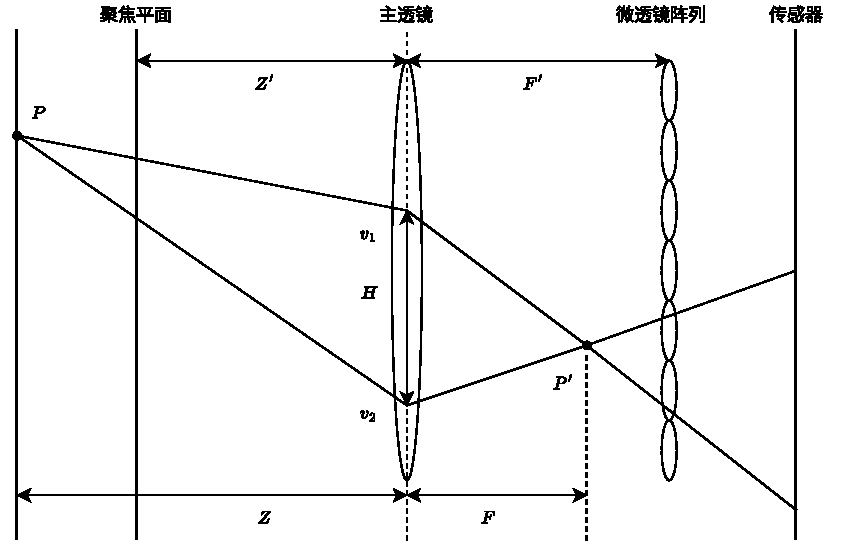
\includegraphics[width=0.80\linewidth]{figures/chapter2/microlens_array_imaging.drawio}
	\bicaption{基于微透镜阵列的光场相机成像原理}
	{Imaging principle of light field camera based on microlens array}  
	\label{cpt2_fig8:multi_array}
\end{figure}

具体来说,如图~\ref{cpt2_fig8:multi_array}~所示,
在观察同一目标$P$时,考虑两个视角 $v_{1}$ 和 $v_{2}$,
目标经过主透镜成像后形成像素点$P'$,
其中目标$P$到主透镜的距离为$Z$,而$Z'$表示主透镜到聚焦平面的距离,
主透镜到成像点的距离为$F$,主透镜到微透镜阵列的距离为$F'$。
两视点之间的距离用$H$表示,由此可推导出如下几何关系:
%
%
\begin{equation}
	\frac{D}{H} = \frac{F'}{Z'} - \frac{F'}{Z} 
	\label{cpt2_fac1:relate}
\end{equation}
%
%
其中$D$表示视差,$F'$、$H$和$Z'$都是相机内参,用来计算目标$P$点的深度。\par
%
%

%
%
%
%
从公式~\ref{cpt2_fac1:relate}~可以看出,
%深度与多视角之间存在密切关系,根据这些关系建模是当前基于多视角图像的显著性目标检测的重要研究方向。
在深度模型中引入场景结构线索是当前基于多视角图像的显著性目标检测研究的重点之一。
%根据公式 2.4 揭示的关系,在深度模型中引入场景结构线索是当前基于多视角图像的显著性目标检测研究的重点之一。
其中,MAC~\cite{zhang2020light}是一项具有代表性的工作,
它通过将微透镜图像阵列输入端到端的卷积神经网络中,
首先对单视点图像的角度变化进行建模,然后将提取的特征输入到现有网络模型中,以捕获多尺度和长程空间依赖信息。
%
%
%此外,类似的方法还包括 DLSD[24],它将光场显著性目标检测任务拆分为两个子任务:通过合成多视角图像来定位显著性目标。这些方法通过利用视差和多视角图像之间的关系完成合成光场的任务。
%
此外,还有像DLSD~\cite{piao2019deep}这样的方法,
它将光场显著性目标检测分解为两个部分:
一个是从中心视角图像生成多视角光场图像,
另一个是从合成的多视角图像中定位显著性目标。
这些方法通过利用视差和多视角图像之间的关联来成功完成合成光场的任务。
%
%
%\textcolor{red}{TODO}
%
%
%
%
%
%深度与多视角之间存在密切关系,根据这些关系建模是当前基于多视角图像的显著性目标检测的重要研究方向。一项具有代表性的工作是 MAC,该方法将微透镜图像阵列输入端到端的卷积神经网络中,首先对每个单视点图像的角度变化进行建模,然后将提取的特征输入到现有网络模型中,以捕获多尺度和长程空间依赖信息。此外,还有一些方法,如 DLSD,将光场显著性目标检测分解为两个子任务,合成多视角图像以定位显著性目标。通过利用视差与多视角图像的关系来完成合成光场的任务。




张等研究者~\cite{zhang2022exploring}~所提出的 ESCNet网络,
将光场显著性检测重新构造成为两个子问题:
从单个视图中进行光场合成和基于光场的显著性目标检测。
即先用一个高质量的光场合成网络,生成可靠的4D光场信息,
在利用多个视点之间的空间相关性,构造基于信息整合光场显著性目标检测网络。

















%%%%%%%%%%%%%%%%%%%%%%%%%%%%%%%%%%%%%%%%%%%%%%%%%%%%%%%%%%%%%%%%%%%%%%%%%%%%
\BiSubsection{基于焦点堆栈的显著性目标检测原理}
{Principles of Salient Object Detection via Focus Stack}
%
%
%
%
目前,以焦点堆栈数据为基础进行显著性目标检测是光场显著性目标检测的主要趋势。
这种方法主要依赖于多焦特性,即场景聚焦于焦点堆栈中不同深度的目标,
%以增强在复杂场景下的显著性检测效果,
%这一方法旨在通过多样性利用焦点堆栈中不同深度的聚焦特性,
通过探索其中蕴藏的场景结构信息,
以提高显著性检测的精确性和鲁棒性。
% 该方法专注于利用不同深度的多焦特性,旨在提升显著性目标检测在复杂场景中的性能表现。
\par 
%
%
%
%
传统光场显著性目标检测方法使用焦点堆栈依赖手动处理的低级特征。
它们首先对输入图像进行超像素分割,然后编码焦点堆栈的聚焦度量线索,
并结合先验知识定位显著性目标。
本文通过LFS~\cite{li2014saliency}模型详细介绍这一原理。
在LFS中,通过计算不同切片间的结构相似性来获得聚焦度量,结合位置先验知识识别背景和前景切片。
接着,在全聚焦图像中计算背景先验和对比度,生成粗略的显著性图。
最后,将粗糙显著性图与前景切片的粗糙显著性图合并。
在合并过程中,通过对焦点堆栈数据进行频域分析,利用高斯滤波计算每个切片的物体性,
对全聚焦支路和前景切片支路的粗糙显著性预测图进行加权,生成最终的预测图。
总的来说,传统基于焦点堆栈的方法仍然倚赖手动处理的低级特征,
利用焦点堆栈的多聚焦特性来选择适当的前景切片,从而完成显著性目标的定位。\par
%
%
%
%
基于深度学习的焦点堆栈显著性目标检测模型通过特征提取和特征融合两个阶段来实现显著性检测。
如图~\ref{cpt2_fig9:model_of_fs_inputs}~中所示,
在特征提取阶段,利用编码器从全聚焦图像和焦点堆栈中提取低阶特征和高阶特征;
而在特征融合阶段,通过采用注意力机制\cite{zhang2021learning}或ConvLSTM\cite{zhang2019memory}对焦点堆栈特征和全聚焦图像特征进行加权求和,实现跨模态的特征融合。最终,经过一层卷积层和Sigmoid层处理后得到最终预测结果。
目前的研究多致力于在特征融合阶段探索更为有效的特征整合策略,以提高检测性能。
%
%
%基于焦点堆栈数据进行显著性目标检测是当前光场显著性目标检测的主流方向。主
%要是依赖焦点堆栈中聚焦于不同深度的多聚焦特性,挖掘其中存在的场景结构信息以提高复杂场景下的显著性检测性能。
%
%传统的基于焦点堆栈的光场显著性目标检测依赖手工低阶特征,先对输入图像进行
%超像素分割,将焦点堆栈聚焦度量线索编码,与先验知识相结合定位显著性目标。本文
%通过 LFS[43]模型阐述传统基于焦点堆栈的光场显著性目标检测的原理。在 LFS 中,首先
%通过计算焦点堆栈不同切片之间的结构相似性得到聚焦度度量,将聚焦度度量与位置先
%验知识相结合,确定背景切片与前景切片。之后,在全聚焦图像中计算背景先验以及对
%比度,获取粗糙的显著性图。最后将粗糙的显著性图与前景切片的粗糙显著性图合并,
%在合并过程中,通过对焦点堆栈数据进行频域分析,使用高斯滤波计算每个切片的物体
%性,对全聚焦支路以及前景切片支路的粗糙显著性预测图进行加权,生成最终的预测图。
%从上述工作表示可以看出,传统的基于焦点堆栈的方法仍然依赖手工低阶特征,利用焦
%点堆栈的多聚焦特性,挑选出合适的前景切片,完成显著性目标的定位。
%基于深度学习的焦点堆栈显著性目标检测模型通过特征提取与特征融合两部分完
%成显著性检测。如图 2.10 所示,在特征提取部分,将全聚焦图像与焦点堆栈输入至编码
%器获取低阶特征和高阶特征,在特征融合部分,采用注意力机制或者 ConvLSTM 对焦
%点堆栈特征以及全聚焦图像特征进行加权求和,完成跨模态的特征整合。最后经过一层
%卷积层以及 Sigmoid 层得到预测结果。当前方法大多致力于在特征融合分布探索更有效
%的特征整合策略。
%
%
\begin{figure}[!ht]
	\centering
	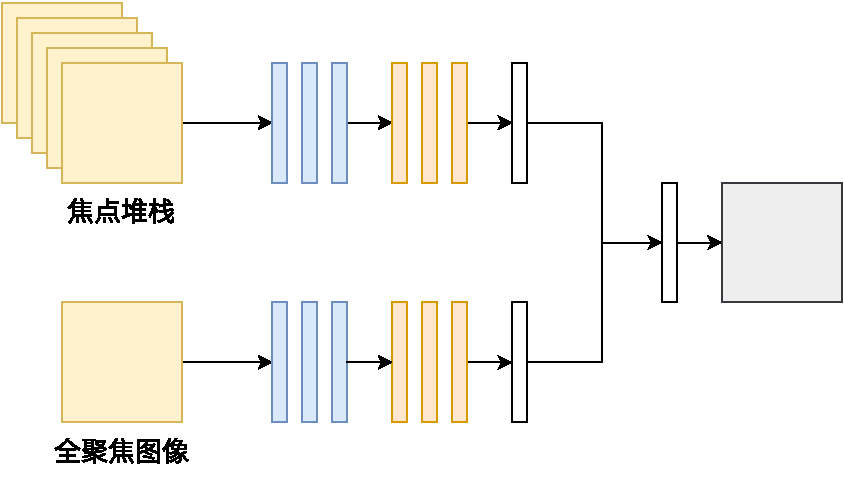
\includegraphics[width=0.80\linewidth]{figures/chapter2/model_of_fs_inputs}
	\bicaption{基于焦点堆栈的光场显著性目标检测模型}
	{Light field salient object detection model based on focus stack}  
	\label{cpt2_fig9:model_of_fs_inputs}
\end{figure}





%%%%%%%%%%%%%%%%%%%%%%%%%%%%%%%%%%%%%%%%%%%%%%%%%%%%%%%%%%%%%%%%%%%%%%%%%%%%
\BiSection{显著性目标检测性能评估指标}
{Performance Evaluation Metrics for Salient Object Detection}



为了全面评估各种显著性目标检测模型在不同数据集上的分割性能,
本节将介绍显著性目标检测任务中广泛使用的五种评估指标。
分别包括
平均绝对误差(Mean Absolute Error,MAE)、
精确率-召回率曲线(P-R曲线)、
F-measure\cite{achanta2009frequency}、
加权的F-measure\cite{margolin2014evaluate}、
E-measure~\cite{fan2018enhanced}和
S-measure~\cite{fan2017structure}。\par






%%%%%%%%%%%%%%%%%%%%%%%%%%%%%%%%%%%%%%%%%%%%%%%%%%%%%%%%%%%%%%%%%%%%%%%%%%%%%%%
(1)平均绝对误差\par
平均绝对误差通过衡量显著性预测图与相应的真实值之间的平均每个像素点绝对差异来
直观的评估显著性图的质量。
它是评估预测质量的最简单有效的方式。
该评估指标的公式如下:
\begin{equation}
	MAE=\frac{1}{W \times H}\sum_{i=1}^{W} \sum_{j=1}^{H} \left |  \hat{S} (i,j) - S(i,j)\right | 
\end{equation}
%
%
其中$\hat{S}(i,j)$和$S(i,j)$分别表示显著性预测图和相应真值图对应坐标的像素。
值得一提的是,当该性能指标的值越低时,意味着预测图越接近真值图。
平均绝对误差展现了出色的可解释性,因为它直接展示了模型预测值与实际值之间的差异大小,
有助于让研究者更加直观地评估模型的性能。
需要留意的是,平均绝对误差对异常值比较敏感,因为它会均等对待每个样本的误差。
若数据集包含异常值,这将会对平均绝对误差的计算结果造成较大影响。



%%%%%%%%%%%%%%%%%%%%%%%%%%%%%%%%%%%%%%%%%%%%%%%%%%%%%%%%%%%%%%%%%%%%%%%%%%%%%%%
(2)精确率-召回率曲线(P-R曲线)\par
%
%
P-R 曲线是用来评估预测图的精准率和召回率的工具。
%P-R曲线就是精确率和召回率的曲线,
曲线以召回率作为横坐标轴,以精确率作为纵坐标轴。
在评估二分类任务时,通常会构造混淆矩阵加以分析,
精确率和召回率可以从混淆矩阵中计算而来,公式如下:
%
%
\begin{equation}
	Precision = \frac{TP}{TP + FP},~Recall = \frac{TP}{TP+FN}
\end{equation}
%
%
其中分类器把正例正确地分类为正例,表示为TP(true positive),
把正例错误地分类为负例,表示为FN(false negative),
把负例正确地分类为负例,表示为TN(true negative),
把负例错误分类为正例,表示为FP(false positive)。
% 那么P-R曲线是怎么来的呢?
算法对样本进行分类时,都会有置信度,即表示该样本是正样本的概率,
比如0.99的概率认为样本A是正例,0.01的概率认为样本B是正例。
通过选择合适的阈值,比如以0.5为阈值对样本进行划分,
预测置信度大于0.5的就认为是正例,小于0.5的就是负例。
通过置信度就可以对所有样本进行排序,再逐个样本的选择阈值,
在该样本之前的都属于正例,该样本之后的都属于负例。
每一个样本作为划分阈值时,都可以计算对应的Precision和Recall,
那么就可以以此绘制P-R曲线。\par




%%%%%%%%%%%%%%%%%%%%%%%%%%%%%%%%%%%%%%%%%%%%%%%%%%%%%%%%%%%%%%%%%%%%%%%%%%%%%%%
(3)
F-measure



F-measure是通过精确度和召回率的加权调和均值来计算的。
P-R~曲线评估分类精度的方法需要在对预测图的每个像素进行二值化后,根据不同的阈值进行比较。
阈值的变化会导致评估精度出现波动。
为了综合考虑精准率和召回率之间的关系,
研究者提出了 F-measure,该指标同时考量了精准率与召回率。
评估指标的公式如下:
%
%
\begin{equation}
	F_{\beta} = \frac{\left ( 1 + \beta^{2} \right ) \times Precision \times Recall }{\beta^{2} \times Precision + Recall } 
\end{equation}
%
%
在上述公式中,Precision 和 Recall 分别代表精准率和召回率。
它们采用了自适应阈值以避免评估过程中的波动,其中$\beta$表示精准率和召回率之间的权重,
通常将$\beta^{2}$设置为 0.3。
该性能指标的越高表示预测结果越好。
F-measure之所以受人青睐在于其综合考量了精确率和召回率,
因此在处理一些不平衡的数据集和样本分布较为复杂的情况下具有很好的适用性。
然而,由于F-measure对于精确率和召回率的平衡要求较高,
可能在某些情况下导致难以准确评估模型的性能。






%%%%%%%%%%%%%%%%%%%%%%%%%%%%%%%%%%%%%%%%%%%%%%%%%%%%%%%%%%%%%%%%%%%%%%%%%%%%%%%
(4)
加权的F-measure\par
%
%
加权F-measure克服了依赖缺陷、等重要缺陷和插值缺陷\cite{margolin2014evaluate}。也是评估显著性预测图时经常会使用的评价指标。其公式如下:
\begin{equation}
	F_{\beta}^{w} = \frac{\left ( 1 + \beta^{2} \right ) \times Precision^{w}  \times Recall^{w} }{\beta^{2} \times Precision^{w} + Recall^{w} } 
\end{equation}
%
%
其中$w$是基于欧几里得距离的加权函数。
加权F-measure综合考虑了模型在不同类别上的性能表现,
对于不同类别样本数量不同的情况也很合适。
一般而言,加权F-measure相比简单平均F-measure更准确地评估了模型的性能。
加权F-measure的数值越高,意味着模型性能越好。







%%%%%%%%%%%%%%%%%%%%%%%%%%%%%%%%%%%%%%%%%%%%%%%%%%%%%%%%%%%%%%%%%%%%%%%%%%%%%%%
(5)
E-measure\par
%
%
E-measure~是一项新近提出的性能评价指标,
综合考虑了显著性预测图与真值图在全局和局部上的相似性,
弥补了以往评价指标只关注单个像素预测精度的缺陷。
E-measure~通过评估局部像素信息与全局均值之间的差异来评价预测结果和真值的像素一致性。
具体评估指标公式如下:

\begin{equation}
	E_{\phi } = \frac{1}{w \times h} \sum_{i=1}^{w} \sum_{j=1}^{h} \phi\left ( i,~j \right ) 
\end{equation}
%
%
%
%
其中$\phi\left (\cdot \right ) $代表增强的对齐矩阵,
在需要比较的两幅图像高度相似时,
其值较大,$w$和$h$表示图像的尺寸。
该性能指标数值越高,意味着显著性预测结果越好。
E-measure展现了良好的稳定性和解释性,
有助于对显著性目标检测等图像分割算法的性能进行相对准确的评估。
然而,它对误差容忍度和边缘细化系数的选择相当敏感,
因此需要根据具体情况进行调整。
另外,E-measure仅适用于二值图像分割问题,
无法直接用于其他类型的分割问题。



(6)
S-measure\par
%
%
%
S-measure 的提出旨在评估显著性图与真值之间的结构相似性,
它弥补了以往评价指标在物体结构上评估能力不足的缺陷。
该评估方法综合考虑了区域级和对象级的相似度。
区域级相似度是通过对各区域的结构相似性度量(Structural Similarity,~SSIM)进行加权求和得到的,
而对象级相似度则是通过比较预测图像与显著性标签的前景区域和背景区域的相似性来确定的。
S-measure 的评估指标公式如下所示:
\begin{equation}
	S_{\alpha} = \alpha * S_{o} + \left ( 1 - \alpha  \right )*S_{r} 
\end{equation}
%
%
其中,$S_{o}$代表对象级的结构相似性,$S_{r}$代表区域级的结构相似性,
而$\alpha$则用于平衡$S_{o}$和$S_{r}$的影响。
通常来说,根据Fan等人~\upcite{fan2018enhanced}的设定,
$\alpha$被设定为0.5。
很显然,对于与真值越接近的显著性预测图,S-measure值就越高。
%
%




%%%%%%%%%%%%%%%%%%%%%%%%%%%%%%%%%%%%%%%%%%%%%%%%%%%%%%%%%%%%%%%%%%%%%%%%%%%%
\BiSection{本章小节}{The Chapter’s Conclusion}

本章首先阐述了光场技术的基本理论,介绍了光场的成像原理以及数据可视化形式;
然后介绍了光场显著性目标检测的相关理论,分别描述了基于多视角图像的显著性目标检测、
基于焦点堆栈的显著性目标检测方法的实现原理,
并引入了显著性目标检测中常用的几种性能评价指标。